\section{Applications and Results of the Developed Framework}

\subsection{Integration of Concepts}
\textcolor{red}{What happens here is to bring the simulated data into a format that is compatible with my analysis of the real-life events data.}
 \begin{figure}[!ht]
	\begin{center}
		\makebox[\textwidth]{
			\centering
			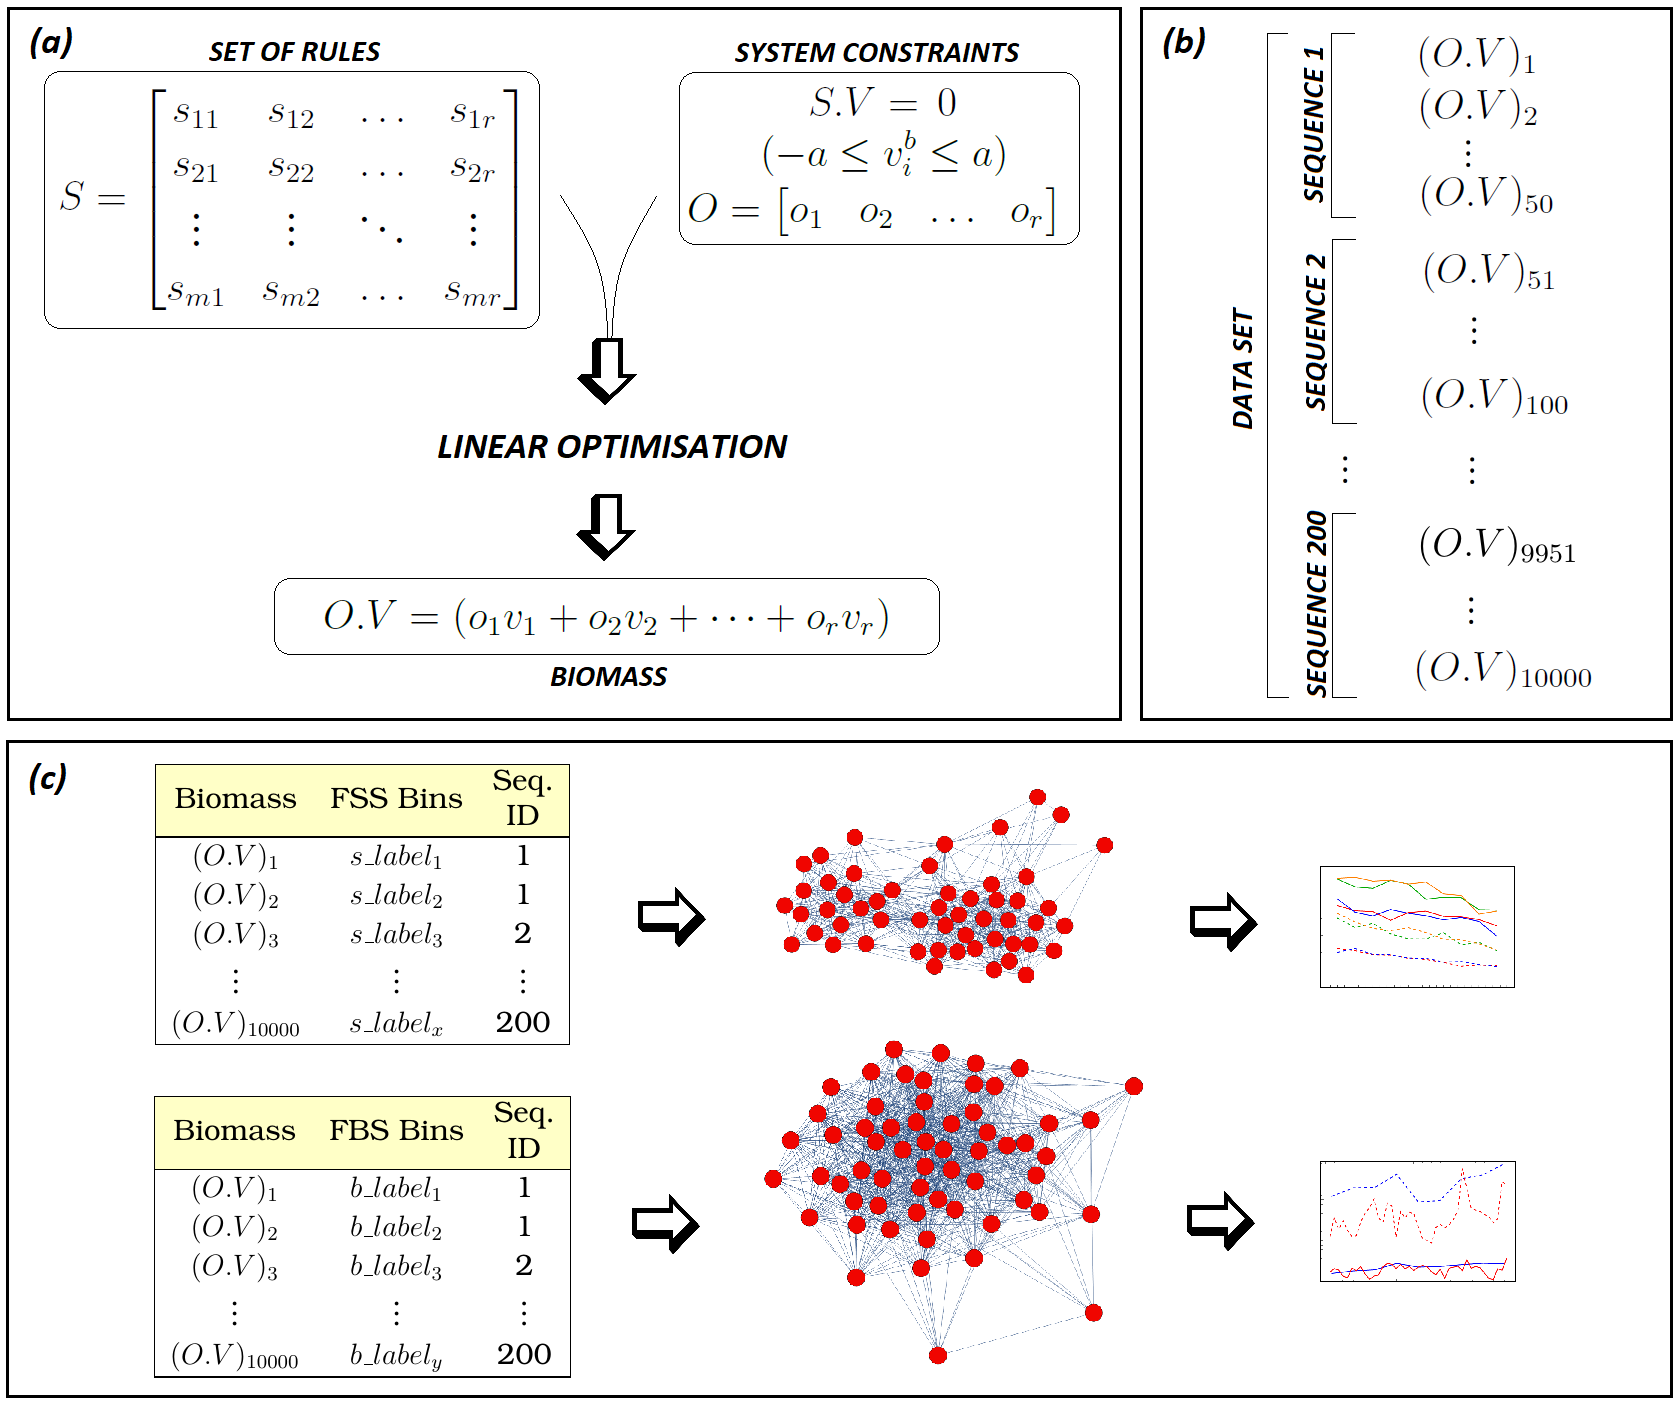
\includegraphics[width=1\linewidth]{../images/methodology-ORmodel-cartoon_complete_framework.png}}
		\caption{Simulation Model Illustration}
		\label{figure-complete_framework_cartoon}
	\end{center}
\end{figure}

%\begin{table}[hb!]
%	\centering
%	\setlength{\arrayrulewidth}{0.5pt}% 
%	\begin{tabular}{|ccc|}
%		\hline \rowcolor[HTML]{FFFFC7}
%		Biomass & FSS Bins	& \makecell{Seq.\\ID}  	\\ \hline
%		$(O.V)_{1}$	    & $s\_label_{1}$	& 1 		\\
%		$(O.V)_{2}$	    & $s\_label_{2}$	& 1 		\\
%		$(O.V)_{3}$	    & $s\_label_{3}$	& 2 		\\
%		\vdots  		& \vdots		& \vdots 	\\
%		$(O.V)_{10000}$	& $s\_label_{x}$	& 200 		\\ \hline
%	\end{tabular}
%\end{table}
%\begin{table}[hb!]
%	\centering
%	\setlength{\arrayrulewidth}{0.5pt}% 
%	\begin{tabular}{|ccc|}
%		\hline \rowcolor[HTML]{FFFFC7}
%		Biomass & FBS Bins	& \makecell{Seq.\\ID}  	\\ \hline
%		$(O.V)_{1}$	    & $b\_label_{1}$	& 1 		\\
%		$(O.V)_{2}$	    & $b\_label_{2}$	& 1 		\\
%		$(O.V)_{3}$	    & $b\_label_{3}$	& 2 		\\
%		\vdots  		& \vdots		& \vdots 	\\
%		$(O.V)_{10000}$	& $b\_label_{y}$	& 200 		\\ \hline
%	\end{tabular}
%\end{table}

%\begin{equation} %\tag{8}
%	(O.V)_{1}= (o_{1,1}v_{1} + o_{1,2}v_{2} + \dots + o_{1,r}v_{r})
%\end{equation}

%\begin{equation} %\tag{8}
%	(O.V)_{2}= (o_{2,1}v_{1} + o_{2,2}v_{2} + \dots + o_{2,r}v_{r})
%\end{equation}

%\begin{equation} 	
%	(O.V)_{50}= (o_{50,1}v_{1} + o_{50,2}v_{2} + \dots + o_{50,r}v_{r})
%\end{equation}

%\begin{equation} 	
%	(O.V)_{51}= (o_{1,1}v_{1} + o_{1,2}v_{2} + \dots + o_{1,r}v_{r})
%\end{equation}

%\begin{equation} 	
%	(O.V)_{100}= (o_{50,1}v_{1} + o_{50,2}v_{2} + \dots + o_{50,r}v_{r})
%\end{equation}

%\begin{equation} 	
%	(O.V)_{10000}= (o_{50,1}v_{1} + o_{50,2}v_{2} + \dots + o_{50,r}v_{r})
%\end{equation}

\subsection{Simulation Results}
{\color{red} 
	
	Briefly explain \emph{in silico analyses} attempts /numerical experiments from the generated data.
	
}



%\begin{equation} %\tag{8}
%	(O.V)_{1}= (o_{1,1}v_{1} + o_{1,2}v_{2} + \dots + o_{1,r}v_{r})
%\end{equation}

%\begin{equation} %\tag{8}
%	(O.V)_{2}= (o_{2,1}v_{1} + o_{2,2}v_{2} + \dots + o_{2,r}v_{r})
%\end{equation}

%\begin{equation} 	
%	(O.V)_{50}= (o_{50,1}v_{1} + o_{50,2}v_{2} + \dots + o_{50,r}v_{r})
%\end{equation}

%\begin{equation} 	
%	(O.V)_{51}= (o_{1,1}v_{1} + o_{1,2}v_{2} + \dots + o_{1,r}v_{r})
%\end{equation}

%\begin{equation} 	
%	(O.V)_{100}= (o_{50,1}v_{1} + o_{50,2}v_{2} + \dots + o_{50,r}v_{r})
%\end{equation}

%\begin{equation} 	
%	(O.V)_{10000}= (o_{50,1}v_{1} + o_{50,2}v_{2} + \dots + o_{50,r}v_{r})
%\end{equation}

%\begin{table}[hb!]
%	\centering
%	\begin{tabular}{|cccccc|l}
%		\cline{1-6}
%		\makecell{Event\\ID} && \makecell{Bio\\Mass} 	&& \makecell{Seq.\\ID} &  \\ \cline{1-6}
%		1 	      && $m_{1}$  	&& 1 		   	&  \\
%		2 		  && $m_{2}$	&& 1 		   	&  \\
%		3 	      && $m_{3}$	&& 2 		    &  \\
%		\vdots	  && \vdots && \vdots 	    &  \\
%		n 		  && $m_{n}$	&& k 		    &  \\ \cline{1-6}
%	\end{tabular}
%	\caption{Arbitrarily Created Data Set $D$.}
%	\label{Tab:D-dataset}
%\end{table}